\documentclass[../../main.tex]{subfiles}
\begin{document}

\begin{flushright}
\footnotesize\textit{【自動文字起こし・要確認】}
\end{flushright}

{\bf [解]}
$P(\alpha,\sqrt{3}\alpha)$，$Q(\beta,-\sqrt{3}\beta)$とする．この時，
\begin{align}
0\le\alpha\le2,\quad-2\le\beta\le0\quad\cdots①
\end{align}
とする．
\begin{align}
|\overrightarrow{OP}|=2\alpha,\qquad|\overrightarrow{OQ}|=-2\beta
\end{align}
だから題意の条件は
\begin{align}
2(\alpha-\beta)=6\iff\alpha-\beta=3\quad\cdots②
\end{align}
である．この時，直線$PQ$の方程式は
\begin{align}
\ell:\sqrt{3}(\alpha+\beta)(x-\alpha)-(\alpha-\beta)(y-\sqrt{3}\alpha)=0
\end{align}
すなわち
\begin{align}
\ell:\sqrt{3}(\alpha+\beta)x-(\alpha-\beta)y-2\sqrt{3}\alpha\beta=0\quad\cdots③
\end{align}
である．②から，$\alpha=\beta+3$だから，①③に代入して，
\begin{align}
\begin{cases}
0\le\beta+3\le2\ \land\ -2\le\beta\le0\\
\ell:\sqrt{3}(2\beta+3)x-3y-2\sqrt{3}(\beta+3)\beta=0
\end{cases}
\iff
\begin{cases}
-2\le\beta\le-1\\
y=\dfrac{\sqrt{3}}{3}\left\{(2\beta+3)x-2(\beta+3)\beta\right\}=:f(\beta)
\end{cases}\quad\cdots④
\end{align}

まず，④の（$\beta$を動かした時の）動く範囲を求める．
\begin{align}
f(\beta)&=\dfrac{\sqrt{3}}{3}\left(-2\beta^2+(2x-6)\beta+3x\right)\\
&=-\dfrac{2\sqrt{3}}{3}\left[\left(\beta-\dfrac{x-3}{2}\right)^2-\dfrac{x^2+9}{4}\right]
\end{align}

であり，$\beta$の2次関数として上に凸で，頂点は$\beta=\dfrac{x-3}{2}$である．

$0\le x\le1$の時，$\beta$は制限なく$-2\le\beta\le-1$を動き，頂点$\dfrac{x-3}{2}\in[-1.5,-1]\subset[-2,-1]$だから，最大値は$f\left(\dfrac{x-3}{2}\right)$，最小値は$f(-1)$，$f(-2)$のうち小さい方である．
\begin{align}
f(-1)=\dfrac{\sqrt{3}}{3}(x+4),\qquad f(-2)=\dfrac{\sqrt{3}}{3}(-x+4),\qquad f\left(\dfrac{x-3}{2}\right)=\dfrac{2\sqrt{3}}{3}\cdot\dfrac{x^2+9}{4}=\dfrac{\sqrt{3}}{6}(x^2+9)
\end{align}
$0\le x\le1$では$f(-1)\ge f(-2)$だから，最小値は$f(-2)=\dfrac{\sqrt{3}}{3}(4-x)$．

$1\le x\le2$の時，線分$PQ$が$x$座標$x$を通るには$\beta\le x\le\alpha=\beta+3$が必要，つまり$x-3\le\beta\le x$．①の$-2\le\beta\le-1$とあわせて，$\beta$の動く範囲は$x-3\le\beta\le-1$である．頂点$\dfrac{x-3}{2}$はこの時$\ge x-3$かつ（$x\ge1$だから）$\ge-1$なので，範囲$[x-3,-1]$の外側（右）にあり，$f$は$[x-3,-1]$上単調増加．よって最大値は$f(-1)=\dfrac{\sqrt{3}}{3}(x+4)$，最小値は
\begin{align}
f(x-3)=\dfrac{\sqrt{3}}{3}\left(-2(x-3)^2+(2x-6)(x-3)+3x\right)=\dfrac{\sqrt{3}}{3}\left(-2(x-3)^2+2(x-3)^2+3x\right)=\sqrt{3}x
\end{align}

以上から，$0\le s\le2$のとき，
\begin{align}
0\le s\le1\text{の時，}&\ \dfrac{\sqrt{3}}{3}(4-s)\le t\le\dfrac{\sqrt{3}}{6}(s^2+9)\\
1\le s\le2\text{の時，}&\ \sqrt{3}s\le t\le\dfrac{\sqrt{3}}{3}(s+4)
\end{align}

（$s=1$で両者は$t=\sqrt{3}$から$t=\dfrac{5\sqrt{3}}{3}$まで連続的につながる．）

\paragraph{(2)}

問題の設定は$x\to-x$（$P$と$Q$の役割の入れ替え）について対称だから，$D$は$y$軸対称である．よって，$-2\le s\le-1$，$-1\le s\le0$の場合は上の不等式で$s$を$|s|$に置き換えたものになる．まとめると，$D$は
\begin{align}
|x|\le1\text{の範囲では}&\ \dfrac{\sqrt{3}}{3}(4-|x|)\le y\le\dfrac{\sqrt{3}}{6}(x^2+9),\\
1\le|x|\le2\text{の範囲では}&\ \sqrt{3}|x|\le y\le\dfrac{\sqrt{3}}{3}(|x|+4)
\end{align}
で表され（境界を含む），図示すると次のようになる．

\begin{figure}[htb]
\centering
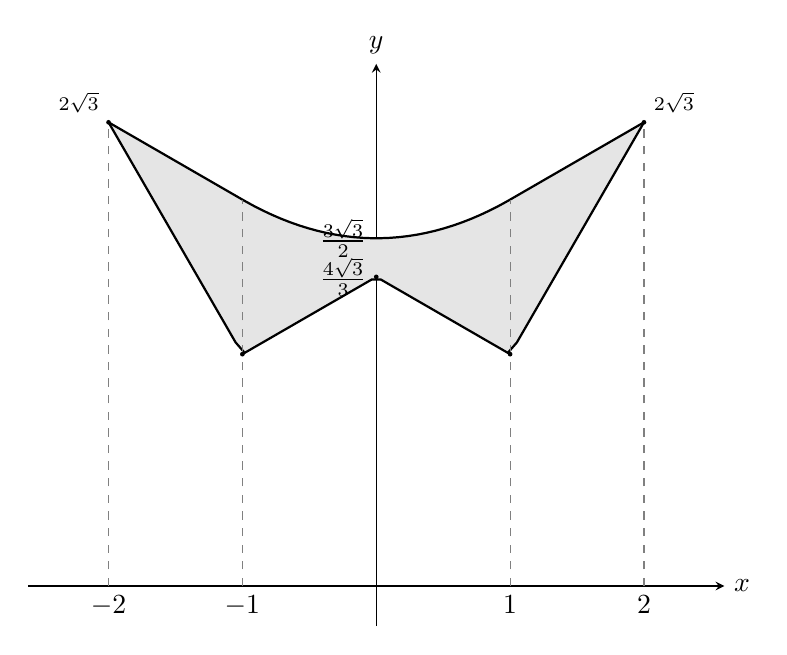
\begin{tikzpicture}[scale=1.7, >=stealth, declare function={
    ftop(\x)=(\x<=1)*(sqrt(3)/6*(\x*\x+9)) + (\x>1)*(sqrt(3)/3*(\x+4));
    fbot(\x)=(\x<=1)*(sqrt(3)/3*(4-\x)) + (\x>1)*(sqrt(3)*\x);
  }]
  \draw[->] (-2.6,0) -- (2.6,0) node[right] {$x$};
  \draw[->] (0,-0.3) -- (0,3.9) node[above] {$y$};
  \fill[gray!20] plot[domain=-2:2,samples=60] (\x,{ftop(abs(\x))}) -- plot[domain=2:-2,samples=60] (\x,{fbot(abs(\x))}) -- cycle;
  \draw[thick] plot[domain=-2:2,samples=60] (\x,{ftop(abs(\x))});
  \draw[thick] plot[domain=-2:2,samples=60] (\x,{fbot(abs(\x))});
  \draw[dashed,gray] (-2,0) -- (-2,{2*sqrt(3)}) (2,0) -- (2,{2*sqrt(3)}) (-1,0) -- (-1,{5*sqrt(3)/3}) (1,0) -- (1,{5*sqrt(3)/3});
  \node[below] at (-2,0) {$-2$};
  \node[below] at (-1,0) {$-1$};
  \node[below] at (1,0) {$1$};
  \node[below] at (2,0) {$2$};
  \node[left] at (0,{4*sqrt(3)/3}) {$\frac{4\sqrt{3}}{3}$};
  \node[left] at (0,{3*sqrt(3)/2}) {$\frac{3\sqrt{3}}{2}$};
  \fill (0,{4*sqrt(3)/3}) circle (0.5pt);
  \fill (-1,{sqrt(3)}) circle (0.5pt);
  \fill (1,{sqrt(3)}) circle (0.5pt);
  \fill (-2,{2*sqrt(3)}) circle (0.5pt);
  \fill (2,{2*sqrt(3)}) circle (0.5pt);
  \node[above right] at (2,{2*sqrt(3)}) {\scriptsize$2\sqrt{3}$};
  \node[above left] at (-2,{2*sqrt(3)}) {\scriptsize$2\sqrt{3}$};
\end{tikzpicture}
\caption{$D$の図示（斜線部，境界を含む）}
\end{figure}

\end{document}
